\documentclass[my_thesis.tex]{subfiles}

\begin{document}
\chapter{The Stepped Pressure Equilibrium Code}\label{ch3.SPEC}

The SPEC code has been developed in the past decade to solve the MRxMHD equilibrium equations (see section \ref{section mrxmhd}); in 2012, \citep{Hudson2012} published a first version that computes fixed-boundary, stepped-pressure equilibria. Since then, it has been upgraded to allow free-boundary calculations \citep{Hudson2020c} and to allow the prescription of the net toroidal current profile \citep{Baillod2021} --- the implementation of this constraint is explained in more details in section \ref{sec. current constraint}. The numerical robustness of the code was and is still continuously improved --- \citep{Qu2020} improved the radial discretization and the numerical solvers in the inner volume of the plasma, and a new boundary representation, based on work by \citet{Henneberg2021}, has been implemented; see details in section \ref{sec. angle representation}.

In addition to these numerical developments, SPEC has been extensively used in the past decade to study diverse physics topics. The code has been rigorously verified in stellarator geometry \citep{Loizu2016}, and has been successfully applied to study current sheets at rational surfaces \citep{Loizu2015,Loizu2015a,Huang2021}, tearing mode stability \citep{Loizu2019} and nonlinear tearing saturation \citep{Loizu2020}, equilibrium $\beta$-limits in a classical stellarator \citep{Loizu2017}, the penetration and amplification of resonant magnetic perturbations in the ideal limit \citep{Loizu2016}, and relaxation phenomenon in reversed field pinches such as the formation of helical states \citep{Dennis2013a} or the relaxation of flow during sawteeth \citep{Dennis2014,Qu2020}. 

%\ac{MRxMHD} has also been extended theoretically to study two-fluid effects \citep{Lingam2016}, and time evolution \citep{Dewar2015,Dewar2017a,Dewar2020}.

In this chapter, an overview of the SPEC code is given. In section \ref{sec. spec_algorithm} some important parts of SPEC algorithm are explained. In section \ref{sec. current constraint} the implementation of the net toroidal current constraint is exposed (see \citep{Baillod2021} for the peer-reviewed publication on that topic). Section \ref{sec. angle representation} discusses some of SPEC numerical issues and how the implementation of a new angle representation is a step towards improving SPEC robustness. Finally, section \ref{sec. chap3 - conclusion} concludes the chapter with some summarizing remarks.

\section{SPEC algorithm \label{sec. spec_algorithm}} 

\subsection{Inputs}
We describe here what are the degrees of freedom in a fixed- and free-boundary SPEC equilibrium. Using the standard cylindrical coordinate system $(R,\phi,Z)$, a plasma boundary surface $\Gamma_{PB}$ is parameterized by $R(\theta,\phi),\ Z(\theta,\phi)$, where $\theta$ is an as of yet undetermined poloidal angle. Toroidal surfaces can be written as double Fourier series, thereafter named the \emph{standard representation},
\begin{align}
	{R}(\theta,\phi) &= \sum_{m=0}^{M_{pol}}\sum_{n=-N_{tor}}^{N_{tor}} R_{mn}\cos(m\theta-nN_{fp}\phi) \label{eq.toroidal surface 1}\\
	{Z}(\theta,\phi) &= \sum_{m=0}^{M_{pol}}\sum_{n=-N_{tor}}^{N_{tor}} Z_{mn}\sin(m\theta-nN_{fp}\phi) \label{eq.toroidal surface 2},
\end{align}
where $M_{pol}$ and $N_{tor}$ are the maximum poloidal and toroidal mode numbers respectively, $R_{mn}$ and $Z_{mn}$ are the Fourier modes of $R$ and $Z$ respectively, $N_{fp}$ is the number of field periods (discrete symmetry) of the system, and $(\theta,\phi)$ are the poloidal and toroidal angles. Note that we assumed stellarator symmetry \citep{pfefferleEnergeticIonDynamics2015} to lighten the notation.

A fixed-boundary \ac{SPEC} equilibrium is then determined by $\Gamma_{PB}$, which is parametrized by the harmonics $(R^{PB_{mn}},Z^{PB_{mn}})$, the number of volumes $N_{vol}$ and the toroidal flux they enclose $\{\psi_{l}\}_{l=\{1,\ldots,N_{vol}\}}$, the pressure in each volume $\{p_l\}_{l=\{1,\ldots,N_{vol}\}}$, the net toroidal  current flowing at the volumes' interfaces $\{I^s_{\phi,l}\}_{l=\{1,\ldots,N_{vol}-1\}}$ and the net toroidal current flowing in each volume $\{I^v_{\phi,l}\}_{l=\{1,\ldots,N_{vol}\}}$.
Note that \ac{SPEC} can be run with different constraints, for example by constraining the toroidal, poloidal and constraint $\mu$ in each volume, $(\psi_{t,l},\psi_{p,l},\mu_l)$, or by constraining the toroidal flux in each volume and the rotational transform on each side of the volume's interfaces $(\psi_{t,l},\iota_-,\iota_+)$. As an output of a fixed-boundary calculation, \ac{SPEC} gives the magnetic field in each plasma volume as well as the geometry of each interface.

A free-boundary equilibrium is determined by a computational boundary surface $\Gamma_{CB}$ surrounding the plasma and enclosed by the coils. This boundary is parametrized by the harmonics $(R^{CB_{mn}},Z^{CB_{mn}})$, according to Eqs.(\ref{eq.toroidal surface 1})-(\ref{eq.toroidal surface 2}). This boundary is in general not a magnetic surface, thus $\mathbf{B}\cdot\mathbf{n}\ne 0$, with $\mathbf{n}=\mathbf{e}_\theta\times\mathbf{e}_\phi$ a vector normal to the computational boundary. The magnetic field is the sum of the magnetic field produced by the coils $\mathbf{B}^c$ and by the plasma $\mathbf{B}^p$. To compute the magnetic field inside the vacuum region, the boundary condition $\mathbf{B}\cdot\mathbf{n}$ on $\Gamma_{CB}$ have to be known. The contribution from the coils, $\mathbf{B}^c\cdot\mathbf{n}$ is provided as input, as Fourier harmonics $V_{mn}$, \textit{i.e.}
\begin{equation}
    \mathbf{B}^c\cdot\mathbf{n} = \sum_{n=-N_{tor}}^{N_{tor}}\sum_{m=0}^{M_{pol}} V_{mn} \sin(m\theta-nN_{fp}\phi),
\end{equation}
where $\mathbf{n}=\mathbf{e}_\theta\times \mathbf{e}_\phi$ is a vector normal to $\Gamma_{CB}$, $\mathbf{B}^c$ is the magnetic field produced by the coils, $M_{pol}$ and $N_{tor}$ are respectively the number of poloidal and toroidal Fourier modes used in the calculation, $N_{fp}$ is the number of field periods, and stellarator symmetry has been assumed. The Fourier harmonics $V_{mn}$ can be obtained from the coil geometry and coil currents; changing the coil shapes, coil currents or the computational boundary $\Gamma_{CB}$ will modify the $V_{mn}$ harmonics non-linearly.  

The field produced by the plasma is \textit{a priori} unknown, and an initial guess for the Fourier harmonics $B_{mn}$ of $\mathbf{B}^p\cdot\mathbf{n}$ have to be provided. Then, SPEC will iterate on the $B_{mn}$ until these are consistant with the actual field profuced by the plasma.

Finally, the calculation of a free-boundary equilibrium requires specifying the total coil current flowing through the torus hole, and, as in fixed-boundary calculations, the profiles $\{\psi_{l}\}_{l=\{1,\ldots,N_{vol}-1\}}$,  $\{p_l\}_{l=\{1,\ldots,N_{vol}-1\}}$,  $\{I^s_{\phi,l}\}_{l=\{1,\ldots,N_{vol}-1\}}$ and $\{I^v_{\phi,l}\}_{l=\{1,\ldots,N_{vol}-1\}}$. The pressure and currents in the last region ($l=N_{vol}$) are set to zero, thereby emulating a vacuum region.  As an output of a free-boundary calculation, SPEC gives the plasma boundary geometry $\Gamma_{PB}$ (\textit{i.e.} the geometry of the outer interface of volume $N_{vol}-1$), the magnetic field in each plasma volume as well as in the vacuum region between $\Gamma_{PB}$ and $\Gamma_{CB}$, the total toroidal flux enclosed by $\Gamma_{CB}$, denoted hereafter by $\widehat\Psi\equiv\sum_{l=1}^{N_{vol}} \psi_l$, and the geometry of the interfaces.


%SPEC  will then iterate on the volume's boundary geometries until force balance is found, \textit{i.e.} equation \ref{eq. force balance} is satisfied. The geometrical degrees of freedom are the Fourier modes of the inner interfaces, \textit{i.e.} $(R_{lmn},Z_{lmn})$ with $l\in\{1,\ldots,N_{vol}-1\}$ and of the plasma boundary in case of free-boundary calculations. These modes are packed in a single array for each interface, named $\mathbf{x}_l$.



\subsection{SPEC coordinates and spectral condensation} \label{spec coord and spectral constraints}
%SPEC can run in three different geometries, namely in slab \citep{Loizu2019},  cylindrical \citep{Loizu2016a} and toroidal geometry \citep{Loizu2016}. The coordinates used to describe position are
%
%\begin{equation}
%	\mathbf{x} = \begin{cases}
%		\theta\hat{\mathbf{i}} + \phi\hat{\mathbf{j}} + R\hat{\mathbf{k}} \qquad &\text{in slab geometry},\\
%		R\cos\theta\hat{\mathbf{i}} + R\sin\theta\hat{\mathbf{j}} + \phi\hat{\mathbf{k}} \qquad &\text{in cylindrical geometry},\\
%		R\cos\phi\hat{\mathbf{i}} + R\sin\phi\hat{\mathbf{j}} + Z\hat{\mathbf{k}} \qquad &\text{in toroidal geometry},
%	\end{cases}
%\end{equation}
%where $\{\hat{\mathbf{i}},\hat{\mathbf{j}},\hat{\mathbf{k}}\}$ is the unitary Cartesian basis, $\theta$ is a poloidal angle and $\phi$ is the usual toroidal angle. The geometry of interface $\mathcal{I}_l$, are described by decomposing the coordinates $R$ and $Z$ on a Fourier basis,
%
%\begin{align}
%	R_l(\theta,\phi) &= \sum_{m=0}^{M_{pol}}\sum_{n=-N_{tor}}^{N_{tor}}R_{l,m,n} \cos(m\theta-nN_p\phi)\\
%	Z_l(\theta,\phi) &= \sum_{m=0}^{M_{pol}}\sum_{n=-N_{tor}}^{N_{tor}}Z_{l,m,n} \sin(m\theta-nN_p\phi),
%\end{align}
%where $N_p$ is the number of field periods, $M_{pol}$ and $N_{tor}$ are the poloidal and toroidal mode numbers above which Fourier series are truncated, \textit{i.e.} $m=\{0,\ldots,M_{pol}\}$, $n=\{-N_{tor},\ldots,N_{tor}\}$, and stellarator symmetry has been assumed for simplicity. Between interfaces $l$ and $l+1$, coordinates are constructed by linear interpolation of $(R,Z)_l$ and $(R,Z)_{l+1}$ using a radial-like coordinate $s$. 



SPEC uses toroidal coordinates $(s,\theta,\phi)$, where $s\in[-1,1]$ is a radial-like coordinate. In the volumes, coordinates $\mathbf{x}=R_l(s,\theta,\phi)\mathbf{e}_R+Z_l(s,\theta,\phi)\mathbf{e}_Z$ are constructed by interpolation between the volume's interfaces, \textit{i.e.}
\begin{align}
	R(s,\theta,\phi) &= {R}_l(\theta,\phi) + {R}_{l+1}(\theta,\phi)f_{lmn}(s)\\
	Z(s,\theta,\phi) &= {Z}_l(\theta,\phi) + {Z}_{l+1}(\theta,\phi)f_{lmn}(s),
\end{align}
with $f_{lmn}$ a regularization factor, 
\begin{equation}
	f_{lmn} = \left\{\begin{array}{ll}
	\frac{1+s}{2} & \text{if } l\ne 1 \text{ or } m=0.\\
	\left(\frac{1+s}{2}\right)^m & \text{if } l=1 \text{ and } m\ne0.
	\end{array}\right.
\end{equation}

In SPEC, the toroidal angle $\phi$ is the cylindrical angle, 
\begin{equation}
	\tan\phi = \frac{y}{x},
\end{equation}
with $(x,y)$ the Cartesian coordinates. The choice of poloidal angle, on the other hand, is more complex. In SPEC, a so-called \emph{spectral condensation} \citep{Hirshman1986} is implemented to select the poloidal angle. The idea is to minimize the number of Fourier harmonics required to represent a surface, \textit{i.e.} minimize
\begin{equation}
	M_l = \frac{1}{2}\sum_{m=0}^{M_{pol}}\sum_{n=-N_{tor}}^{N_{tor}} m^\lambda (R_{mn}^2 + Z_{mn}^2), \label{eq.spectral width}
\end{equation}
where only variations tangential to the surface are allowed, $\delta R = R_\theta\delta u$ and $\delta Z = Z_\theta\delta u$, where the $X_i$ designates a derivative of $X$ with respect to $i$ and $\delta u$ is arbitrary, and $\lambda$ is a user input. In SPEC, an additional target is included in the minimization, called the \emph{spectral length} --- its role is to ensure smooth transition between the angles used to represent inner plasma interfaces and the plasma boundary. It is expressed for volume $\mathcal{V}_l$ as 
\begin{equation}
	L_l = \oint\oint\sum_{i=1}^{N_s}\sqrt{[R_l(\theta,\phi)-R_{l-1}(\theta,\phi)]^2 +  [Z_l(\theta,\phi)-Z_{l-1}(\theta,\phi)]^2}d\theta d\phi, \label{eq.spectral length}
\end{equation}
where $N_s$ is the number of radial grid points $s_i$. Finally, the zero of the poloidal angle is constrained to be such that ${Z}_l(\theta=0,\phi)$ is equal to the geometrical center of the interface $Z_{l,0}$, which can be enforced by minimizing
\begin{equation}
	S_l = \frac{1}{2}\oint ({Z}_l(0,\phi) - Z_{l,0})^2 d\phi, \label{eq.spectral zero}
\end{equation}
with
\begin{equation}
	Z_{l,0} = \oint d\theta Z_l(\theta,\phi)\sqrt{R_{l,\theta}(\theta,\phi)^2 + Z_{l,\theta}(\theta,\phi)^2}.
\end{equation}



The target ot minimize is then a linear combination of all angular targets, Eqs.(\ref{eq.spectral width})-(\ref{eq.spectral zero}),
\begin{equation}
	W_{sc} = \sum_{l=1}^{N_{vol}-1} \alpha_lM_l + \beta_lL_l + \gamma_l S_l,
\end{equation}
where $(\alpha_l,\beta_l,\gamma_l)$ are user supplied weights, and $\psi_a$ is the total toroidal flux enclosed by the plasma. One can show that this can be written under the form

\begin{equation}
	\delta W_{sc} = \oint\oint F^{sc}(\theta,\phi) \delta u d\theta d\phi,
\end{equation}
meaning that the minimum of $W_{sc}$ is found for 

\begin{equation}
	F^{sc} = \sum_{m=0}^{M_{pol}} \sum_{n=-N_{tor}}^{N_{tor}} F^{sc}_{mn} \sin(m\theta-nN_{fp}\phi) = 0. \label{eq. spectral constraint}
\end{equation}






\subsection{Beltrami solver} \label{spec beltrami solver}
At the core of SPEC stands the \emph{Beltrami solver}, which finds the magnetic field that satisfies the Beltrami equation (\ref{eq. beltrami}) given the volume geometry and the profiles. The magnetic field is written as the curl of the magnetic vector potential, $\mathbf{B}_l=\nabla\times\mathbf{A}_l$, which is expanded on a Chebyshev-Fourier basis,

\begin{equation}
	A_{l,i} = \sum_{m,n}\sum_{k=0}^{L_{rad}} A_{l,i,k,m,n} T_k(s)\cos(m\theta-nN_p\phi),
\end{equation}
where $L_{rad}$ is the radial resolution, $T_k$ is the Chebyshev polynomial of order $k$ and $i=\{\theta,\phi\}$. Note that gauge freedom is used to set $A_{l,s}=0\ \forall l$. The coefficients $A_{l,i,k,m,n}$ are the vector potential degrees of freedom, packed in a single array $\mathbf{a}_l$.

In each volume $\mathcal{V}_l$ and given $(\mu_l,\psi_{p.l},\psi_{t,l})$, geometry dependent matrices $\mathbf{G}_l$ and $\mathbf{C}_l$ are constructed and used to write the Beltrami equation (\ref{eq. beltrami}) as a linear system,
\begin{equation}
	\mathbf{G}_l[\mathbf{x}_{l-1},\mathbf{x}_l,\mu_l]\mathbf{a_l} = \mathbf{C}_l[\psi_{p,l},\psi_{t,l}]. \label{eq.linearized_beltrami_system}
\end{equation}


If the input profiles are the rotational transform on the inner and outer side of the interfaces $\mathcal{I}_l$, initial guesses for $(\mu_l,\psi_{p,l})$ are used first and iterated upon until the rotational transform constraint is matched. Note that there are some differences for the special case of the inner most volume, which has a different topology (torus instead of an annulus) and for the vacuum region, since $\mathbf{B}\cdot\mathbf{n}\ne 0$ on its outer boundary.




Once this computation is complete, the magnetic field $\mathbf{B}_l$ in agreement with the constraint and the geometry is known in each volume. The next stage is to evaluate the force on each interface $\mathcal{I}_l$.

\subsection{Force solver}
SPEC searches the geometry of the inner plasma interfaces, and of the plasma boundary in case of free-boundary calculations, that minimizes (i) the physical force, \textit{i.e.} Eq.(\ref{eq. force balance}) and (ii) the spectral constraint, \textit{i.e.} Eq.(\ref{eq. spectral constraint}).

The physical force is an even function the poloidal and toroidal angle, and can be written as 
\begin{equation}
	F^{ph}(\theta,\phi) = \left[\left[ p + \frac{B^2}{2\mu_0}\right]\right] = \sum_{m=0}^{M_{pol}}\sum_{n=-N_{tor}}^{N_{tor}} F^{ph}_{mn}\cos(m\theta-nN_{fp}\phi).
\end{equation}

Given the magnetic field in each volume computed by the Beltrami solver, it is trivial to evaluate the magnetic field on a $(\theta,\phi)$ grid on each side of each volume's interface. Taking the difference between the outer and inner side values, and performing a Fourier transformation gives the Fourier harmonics $F^{ph}_{mn}$. All Fourier harmonics of the physical force and of the spectral constraint are packed in a single array, name $\mathbf{F}$.

Finally, SPEC will iterate on $\mathbf{x}_l$ until $\mathbf{F}$ is smaller than a tolerance set by the user. A Powell hybrid method is used, and analytical derivatives of $F_{mn}$ with respect to the interface geometry harmonics $(R_{lmn}, Z_{lmn})$ are provided. Details about their computations are given in the case of the toroidal current constraint in section \ref{sec. force gradient}. The SPEC algorithm is summarized in Figure \ref{fig.spec algorithm complete}.

\begin{figure}
	\centering
	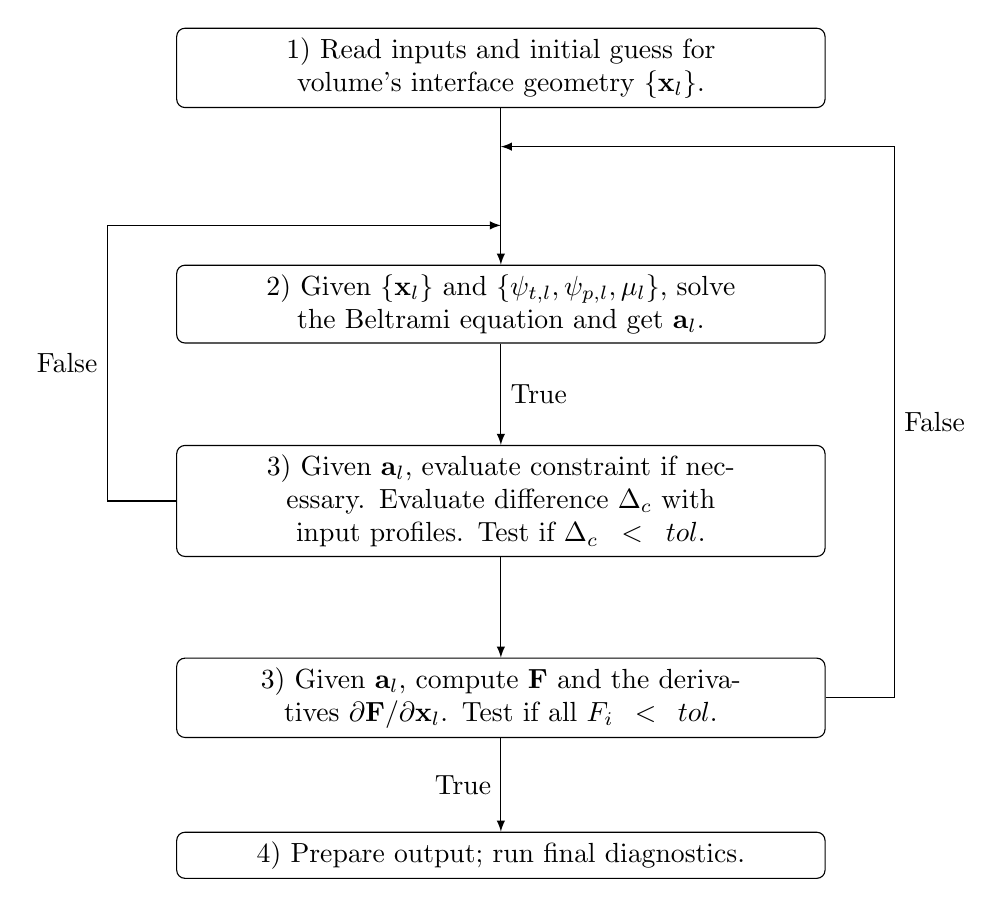
\begin{tikzpicture}
		\tikzstyle{MyAlgoStep}=[draw,text width=8cm,text centered,rounded corners=3pt]
		\node[MyAlgoStep] (init) at (0,6) {
			1) Read inputs and initial guess for volume's interface geometry $\{\mathbf{x}_l\}$.
		};
		\node[MyAlgoStep] (beltrami) at (0,3) { 
			2) Given $\{\mathbf{x}_l\}$ and $\{\psi_{t,l},\psi_{p,l},\mu_l\}$, solve the Beltrami equation and get $\mathbf{a}_l$.
		};
		\draw[->,>=latex] (init.south) -- (beltrami.north);
		\node[MyAlgoStep] (constraint) at (0,0.5) {
			3) Given $\mathbf{a}_l$, evaluate constraint if necessary. Evaluate difference $\Delta_c$ with input profiles. Test if $\Delta_c<\text{tol}$.
		};
		\draw[->,>=latex] (beltrami.south) -- (constraint.north) node[midway,anchor=west] () {True};
		\draw[->,>=latex] (constraint.west) -- (-5,0.5) -- (-5,4) node[midway,anchor=east] () {False} -- (0,4);
		\node[MyAlgoStep] (force) at (0,-2) {
			3) Given $\mathbf{a}_l$, compute $\mathbf{F}$ and the derivatives $\partial \mathbf{F} / \partial \mathbf{x}_l$. Test if all $F_i<\text{tol}$.
		};
		\draw[->,>=latex] (constraint.south) -- (force.north);
		\node[MyAlgoStep] (output) at (0,-4) {
			4) Prepare output; run final diagnostics.
		};
		\draw[->,>=latex] (force.south) -- (output.north) node[midway,anchor=east] () {True};
		\draw[->,>=latex] (force.east) -- (5,-2) -- (5,5) node[midway,anchor=west] () {False} -- (0,5);
	\end{tikzpicture}
	\caption{Main components of SPEC algorithm}
	\label{fig.spec algorithm complete}
\end{figure}

It is worth noting that even though the magnetic helicity is not conserved when \ac{SPEC} iterates on $\{x_i\}_{i=1,\ldots,N}$ to find an equilibrium that matches a given input $\{\psi_{t,l}, \psi_{p,l}, \mu_l\}_{l=1,\ldots,N_{vol}}$ or $\{\psi_{t,l},\ \iotabar_l^+,\  \iotabar_l^-\}_{l=1,\ldots,N_{vol}}$, the final equilibrium satisfies the \ac{MRxMHD} equilibrium equations (Eq.(\ref{eq.BeltramiEquation})-(\ref{eq.force_balance})). There is a magnetic helicity profile $\{K_l\}_{l=1,\ldots,N_{vol}}$ corresponding to this equilibrium which is unknown \textit{a priori}. Thus, the same equilibrium could have been found by minimizing the \ac{MRxMHD} energy functional while keeping the magnetic helicity profile constant if the initial state had the same magnetic helicity profile (bifurcations are not considered in this chapter). This capability is also available in \ac{SPEC}, and details can be found in the literature \citep{Hudson2012,Dennis2013a}.
 

\subsection{Free-boundary iterations}
In case of free-boundary calculations, the magnetic field produced by the plasma on the computational boundary, $\mathbf{B}^p$ is not known \textit{a priori}. This information is however required for the Beltrami solver in the vacuum region to find the magnetic field in agreement with the boundary condition $(\mathbf{B}^p+\mathbf{B}^c)\cdot\mathbf{n}$.

To find self consistent solutions, an additional loop in SPEC is thus required. An initial guess for the Fourier harmonics of $\mathbf{B}^p\cdot \mathbf{n}$, denoted $B_{mn}^0$, is given as input; SPEC finds a solution in agreement with this boundary condition and recompute the harmoncis of $\mathbf{B}^p\cdot\mathbf{n}$, denoted $\tilde{B}_{mn}^1$. Generally, $B_{mn}^0\neq \tilde{B}_{mn}^1$. Thus, a Piccard iteration is performed,

\begin{equation}
	B_{mn}^1 = \alpha B_{mn}^0 + (1-\alpha) \tilde{B}_{mn}^1,
\end{equation}
with $\alpha\in[0,1[$, and SPEC re-evaluate the equilibrium with this new boundary condition. This loop continues until $B_{mn}^i\neq \tilde{B}_{mn}^{i+1}$.


\section{Implementation of toroidal current constraint \label{sec. current constraint}}

The computation of equilibria at fixed toroidal current profile is crucial for basic physic studies \citep{Loizu2017,Suzuki2020}, equilibrium reconstruction \citep{Lao1985,Hanson2009}, and stellarator optimization \citep{Geiger2010,Geiger2015}.  Most \ac{MHD} equilbrium codes (VMEC \citep{Hirshman1983,Hirshman1986}, SIESTA \citep{Hirshman2008,Peraza-Rodriguez2017}, HINT \citep{Harafuji1989,Suzuki2006}, or PIES \citep{Reiman1986,Drevlak2005}) can calculate equilibria at chosen rotational transform or toroidal current profile. \ac{SPEC} could run at fixed rotational transform but only recently its capability to run at fixed toroidal current profile has been implemented. This capability is crucial for studying the effect of toroidal current on 3D magnetic equilibria. Examples are the study of the effect of bootstrap current on equilibrium beta limits, or the study of the sensitivity of a given equilibrium to toroidal current fluctuations. In  this  chapter  we describe the implementation of the  new  capability  for  \ac{SPEC}, that allows \ac{MRxMHD} equilibria to be calculated at prescribed toroidal current profiles.
\subsection{Constraining the toroidal current profiles in \ac{SPEC}}

\ac{SPEC} has been extended to allow the triplet $\{\psi_{t,l}, I^v_{l,\phi}, I^s_{l,\phi}\}_{l=1,\ldots,N_{vol}}$ as a constraint, herein \textit{current constraint}. In the case of the rotational transform constraint, \ac{SPEC} finds the solution to the linear system (\ref{eq.BeltramiEquation}) volume by volume and iterates on $\{\mu_l, \psi_{p,l}\}$ until the field has the desired rotational transform at the volume interfaces. In the case of the current constraint, the constants $\{\mu_l\}_{l=1,\ldots,N_{vol}}$ are determined using Eq.(\ref{eq.volume_current}), without the need for iterations, and this directly constrains the value of volume currents $\{I^v_{l,\phi}\}_{l=1,\ldots,N_{vol}}$.

Regarding the poloidal fluxes, it can be shown  (Appendix \ref{appA1}) that the surface currents depend linearly on the poloidal fluxes, \textit{i.e.} 

\begin{equation}
	\mathbf{I}^s=\mathbf{M}\bm{\psi}_p+\mathbf{Q}\label{eq.complicado},    
\end{equation}
where $\mathbf{I}^s$ and $\bm{\psi}_p$ are arrays containing all $\{I^s_l\}_{l=1,\ldots,N_{vol}-1}$ and all $\{\psi_{p,l}\}_{l=2,\ldots,N_{vol}}$ respectively, and the matrix $\mathbf{M}$ and the  array $\mathbf{Q}$ depend only on the geometry of the interfaces $\{x_i\}_{i=1,\ldots,N}$. In this section, we consider the geometry, toroidal fluxes and the constants $\{\mu_l\}_{l=1,\ldots,N_{vol}}$ to be fixed and seek how the poloidal flux profile $\bm{\psi}_p$ has to be constrained in order to obtain a surface current profile matching the input profile $\mathbf{I}^s$.

The unknown $\mathbf{Q}$ is eliminated by subtracting Eq.(\ref{eq.complicado}) evaluated at two different values of $\bm{\psi}_p$, \textit{i.e.} evaluated once at $\overbar{\bm{\psi_p}}$ and once at $\bm{\psi}_p$,
\begin{equation}
	\mathbf{M} (\overbar{\bm{\psi}_p} - \bm{\psi}_p) = \overbar{\bm{I}^{s}} - \bm{I}^{s}, \label{eq.psip_diff}
\end{equation}
where $\overbar{\bm{\psi}_p}$ is an arbitrary choice of poloidal fluxes, and $\overbar{\bm{I}^s}$ is the surface current profile calculated from the Beltrami fields $\{\overbar{\mathbf{a}_l}\}_{l=1,\ldots,N_{vol}}$ obtained when the poloidal fluxes are constrained to the values $\overbar{\bm{\psi}_p}$.

The matrix $\mathbf{M}$ is evaluated by taking the derivatives of Eq.(\ref{eq.complicado}) with respect to the poloidal fluxes, \textit{i.e.}

\begin{equation}
	M_{ij} = \frac{\partial I^s_{i,\phi}}{\partial \psi_{p,j}},\label{eq.coef_M}
\end{equation}
which leads to the following bi-diagonal matrix

\begin{equation}
	\mathbf{M} = \frac{2\pi}{\mu_0} \begin{bmatrix}\dfrac{\partial \tilde{B}^-_{\theta,2}}{\partial{\psi_{p,2}}} & 0 & \cdots & \cdots  & 0 \\
		-\dfrac{\partial \tilde{B}^+_{\theta,2}}{\partial{\psi_{p,2}}} & \dfrac{\partial \tilde{B}^-_{\theta,3}}{\partial{\psi_{p,3}}} & 0  & \cdots & 0\\
		0 & -\dfrac{\partial \tilde{B}^+_{\theta,3}}{\partial{\psi_{p,3}}} & \dfrac{\partial \tilde{B}^-_{\theta,4}}{\partial{\psi_{p,4}}} & 0  & 0 \\
		\vdots & \ddots & \ddots  & \ddots & 0\\
		0 \cdots  & \cdots & 0 & -\dfrac{\partial \tilde{B}^+_{\theta,N_{vol}-1}}{\partial{\psi_{p,N_{vol}-1}}} & \dfrac{\partial \tilde{B}^-_{\theta,N_{vol}}}{\partial{\psi_{p,N_{vol}}}}\end{bmatrix}.\label{eq.matrix_M}
\end{equation}
Derivatives of $\tilde{B}^\pm_{\theta,l}$ with respect to the poloidal flux can be easily obtained by applying matrix perturbation theory on the linear system (\ref{eq.linearized_beltrami_system}) \citep{Hudson2012},

\begin{equation}
	\mathbf{G}_l \cdot \left[\frac{\partial}{\partial\psi_{p,l}}\mathbf{a}_l\right] = - \left[\frac{\partial}{\partial\psi_{p,l}}\mathbf{G}_l\right] \cdot \mathbf{a}_l + \frac{\partial}{\partial\psi_{p,l}}\mathbf{C}_l.\label{eq.perturbed_matrix}
\end{equation}

Due to the linear nature of Eq.(\ref{eq.complicado}), the coefficients of the matrix $\mathbf{M}$, \textit{i.e.} Eq.(\ref{eq.coef_M}), are independent of $\bm{\psi}_p$ and thus can be evaluated once at any arbitrary value of $\bm{\psi}_p$. We thus conveniently evaluate them at $\overbar{\bm{\psi}_p}$. Equation (\ref{eq.psip_diff}) is then solved to obtain the poloidal flux profile $\bm{\psi}_p$. 

Finally, instead of solving a second time the Beltrami equation, Eq.(\ref{eq.BeltramiEquation}), at $\bm{\psi}_p$, we take advantage of the linear dependence of $\mathbf{a}$ on $\bm{\psi}_p$, Eq.(\ref{eq.linearized_beltrami_system}), and solve  

\begin{equation}
	A_{l,i} = \overbar{A_{l,i}} - \frac{\partial {A_{l,i}}}{\partial {\psi_{p,l}}} (\overbar{\psi_{p,l}} - \psi_{p,l}),\label{eq.NewtonStep_Solution}
\end{equation}
where $\overbar{A_{l,i}}$ is one element of $\overbar{\bm{a}_l}$. The algorithm flow is summarized in Figure \ref{fig.algo_current_constraint}.

\begin{figure}
	\centering
	\begin{tikzpicture}
		\tikzstyle{MyAlgoStep}=[draw,text width=3.5cm,text centered,rounded corners=3pt]
		\tikzstyle{MyBigAlgoStep}=[draw, text width=8cm,text centered,rounded corners=3pt]
		\node[MyBigAlgoStep] (init) at (0,5) {
			1) Set the toroidal flux profile $\{\psi_{t,l}\}_{l=1,\ldots,N_{vol}}$ from input and the constants $\{\mu_{t,l}\}_{l=1,\ldots,N_{vol}}$ using the volume current profile and Eq.(\ref{eq.volume_current})
		};
		\node[draw, thick, dashed] (O) at (0,.7) {
			\begin{minipage}[t][5.8cm]{.95\textwidth}
				\centering
				2) Solve Beltrami equations consistently with the input surface current constraint
			\end{minipage}
		};
		\node[MyAlgoStep] (A) at (-4.5,1.5) {2.1) Chose an arbitrary $\overbar{\bm{\psi_p}}$};
		\node[MyAlgoStep] (B) at (0,1.5) {2.2) Solve Beltrami equation (\ref{eq.BeltramiEquation}) by constraining the poloidal fluxes to the values $\overbar{\bm{\psi_p}}$ to get $\overbar{\mathbf{a}_l}$};
		\node[MyAlgoStep] (C) at (4.5,1.5) {2.3) Solve perturbed matrix equation (\ref{eq.perturbed_matrix}) to get $\dfrac{\partial \overbar{\mathbf{a}_l} }{\partial \psi_{p,l}}$};
		\node[MyAlgoStep] (D) at (4.5,-1) {2.4) Build matrix $\mathbf{M}$ by constructing $\dfrac{\partial \tilde{B}^\pm_{\theta,l}}{\partial \psi_p}$ from $\dfrac{\partial \overbar{\mathbf{a}_l} }{\partial \psi_{p,l}}$};
		\node[MyAlgoStep] (E) at (0,-1) {2.5) Solve equation (\ref{eq.psip_diff}) and get $\bm{\psi_p}$};
		\node[MyAlgoStep] (F) at (-4.5,-1) {2.6) Find $\mathbf{a}$ by solving Eq.(\ref{eq.NewtonStep_Solution})};
		\draw[->,>=latex] (init) -- (O); 
		\draw[->,>=latex] (A) -- (B);
		\draw[->,>=latex] (B) -- (C);
		\draw[->,>=latex] (C) -- (D);
		\draw[->,>=latex] (D) -- (E);
		\draw[->,>=latex] (E) -- (F);
	\end{tikzpicture}
	\caption{Flow of the algorithm used to constrain the net toroidal current profiles for a given toroidal flux profile and geometry.}
	\label{fig.algo_current_constraint}
\end{figure}

In the case of a free-boundary computation, the toroidal flux in the vacuum region is varied to satisfy the poloidal linking current $I_{coil}$. This slightly modifies the linear system (\ref{eq.psip_diff}). Details can be found in Appendix \ref{appA}.

Constraining the toroidal current profile takes away the control of other profiles such as the rotational transform or the magnetic helicity. However, as for the case of the rotational transform constraint, the equilibrium can be accessed by a relaxation process at constant magnetic helicity if the final magnetic helicity is known \textit{a priori}. The \ac{MRxMHD} equations are thus still satisfied by an equilibrium obtained by constraining the toroidal current profiles. 

\subsection{Force gradient}
\label{sec. force gradient}
The hybrid Powell algorithm used in SPEC to iterate on the interfaces geometry uses analytic derivatives, which is faster than finite differentiation. To keep good performance while using the current constraint, derivatives of the force Fourier coefficients, $\{F_j\}_{j=1,\ldots,N}$, with respect to the interfaces degrees of freedom, $\{x_i\}_{i=\{1,\ldots,N\}}$, at constant $\{\psi_{t,l}, I^v_{l,\phi},\ I^s_{l,\phi}\}_{l=1,\ldots,N_{vol}}$ are provided. Derivatives are first evaluated in real space and then Fourier-transformed. Using the chain rule,
\begin{align}
	\frac{d}{d x_i}\left[\left[p + \frac{B^2}{2\mu_0}\right]\right]_l &= \frac{1}{\mu_0}\left( B^-_{l+1}\frac{d B^-_{l+1}}{d x_i} - B^+_l \frac{d B^+_{l}}{d x_i}\right)\\ \label{eq.force_gradient}
	\frac{d B^{\pm}_l}{d x_i} &= \frac{\partial B^\pm_l}{\partial x_i} + \frac{\partial B^\pm_l}{\partial \psi_{p,l}}\frac{d \psi_{p,l}}{d x_i} + \frac{\partial B^\pm_l}{\partial \mu_l}\frac{d\mu_l}{d x_i}+ \frac{\partial B^\pm_l}{\partial \psi_{t,l}}\frac{d\psi_{t,l}}{d x_i}
\end{align}
where $B^-_l$, $B^+_l$ are the magnetic field strength on the inner and outer side of volume $l$, respectively, and the pressure, $p_l$, is considered constant in each volume with respect to variations in the geometry, $\mu_l$ and $\psi_{p,l}$. Note that all derivatives are taken at constant toroidal flux, volume current and surface current. Enforcing $ d\psi_{t,l} / dx_i=0$ and $d I^v_{l,\phi} / dx_i=0$ leads to $d \mu_l/dx_i=0$ using Eq.(\ref{eq.volume_current}). The surface current constraint, $d I^s_{l,\phi}/dx_i=0$, leads to a system of coupled equations using Eq.(\ref{eq.surf_current}),

\begin{equation}
	\frac{\partial \tilde{B}^-_{l+1,\theta}}{\partial x_i} + \frac{\partial \tilde{B}^-_{l+1,\theta}}{\partial \psi_{p,l+1}} \frac{\partial\psi_{p,l+1}}{\partial x_i} - \frac{\partial \tilde{B}^+_{l,\theta}}{\partial x_i} - \frac{\partial \tilde{B}^+_{l,\theta}}{\partial \psi_{p,l}}\frac{\partial\psi_{p,l}}{\partial x_i} = 0, \label{eq.Isurface_derivative}
\end{equation}
which can be written as a linear system using the matrix $\mathbf{M}$ defined in Eq.(\ref{eq.matrix_M}),

\begin{equation}
	\mathbf{M} \cdot  \begin{bmatrix}
		\dfrac{d\psi_{p,2}}{dx_i}\\
		\vdots\\
		\dfrac{d\psi_{p,N_{vol}}}{dx_i}
	\end{bmatrix} = \frac{2\pi}{\mu_0}\begin{bmatrix}
		\dfrac{\partial \tilde{B}^+_{\theta,1}}{\partial x_i} - \dfrac{\partial \tilde{B}^-_{\theta,2}}{\partial x_i} \\
		\vdots \\
		\dfrac{\partial \tilde{B}^+_{\theta,N_{vol}-1} } {\partial x_i} - \dfrac{\partial \tilde{B}^-_{\theta,N_{vol}}}{\partial x_i}
	\end{bmatrix}.\label{eq.linear_system}
\end{equation}
Derivatives of $\tilde{B}_{\theta,l}$ with respect to $\psi_{p,l}$ and $x_i$ can be obtained by applying matrix perturbation theory to the Beltrami system (\ref{eq.linearized_beltrami_system}). The solution of Eq.(\ref{eq.linear_system}), together with Eq.(\ref{eq.force_gradient}) provides the required derivatives of the force with respect to the geometry. Derivatives of the Fourier components of the force, $dF_j/dx_i$, are obtained by taking the Fourier transform of equation (\ref{eq.force_gradient}) and are packed in a matrix $\nabla F$ of size $N^2$, henceforth named \textit{force gradient}. Appendix \ref{appA} provides details on the free-boundary case. 

\subsection{Implementation details and parallelization}
The new current constraint has been parallelized with \ac{MPI} in a similar fashion to the other constraints. Each volume is associated to one \ac{CPU}; since the solution to the Beltrami equation (\ref{eq.BeltramiEquation}) in a volume is independent from other volumes, each \ac{CPU} can solve the linear system (\ref{eq.linearized_beltrami_system}) in parallel. Finally, the master \ac{CPU} gathers all required derivatives to construct the matrix $\mathbf{M}$ and solves the linear system (\ref{eq.psip_diff}), before broadcasting the values of $\{\psi_{p,l}\}_{l=2,\ldots,N_{vol}}$ and $\{\mathbf{a}_l\}_{l=1,\ldots,N_{vol}}$ to all \acp{CPU}.

Regarding communications, we reduced them to a minimum. The global toroidal current constraint is computed using Eq.(\ref{eq.surf_current}), which only depends on the first even Fourier coefficient of $B_\theta$ in each volumes. We thus compute locally (by each \ac{MPI} task) these coefficients before sending them to the master task. This requires the communication of $2(N_{vol}-1)$ doubles. All communications are implemented using basic \ac{MPI} point-to-point communications, though a gathering communication could be more efficient. The master task then solves Eqs.(\ref{eq.psip_diff}) and (\ref{eq.NewtonStep_Solution}) and broadcasts the elements $\overbar{\bm{a}_l}$ and $\overbar{\bm{\psi}_p}$. We don't expect a communication bottleneck due to the reasonably low amount of communications. 

%\subsubsection{Code complexity}
%\label{sec:theoretical_complexity}
%The theoretical complexity of \ac{SPEC} depends on the number of volumes $N_{vol}$ and the radial, poloidal and toroidal resolution $L_{rad}$, $M_{pol}$ and $N_{tor}$ respectively. One of the most time consuming part is the computation of the geometry-dependent matrices. These matrices have $L_{rad}^2\cdot M_{pol}^2\cdot N_{tor}^2$ elements and are computed in each volume. The time spent computing these matrices grows as
%
%\begin{equation}
%	\mathcal{O}_{matrices} \sim \mathcal{O}(N_{vol} L_{rad}^2 M_{pol}^2 N_{tor}^2).
%\end{equation}
%These matrices are evaluated each time the geometry is changed, which depends on the sought equilibrium. Another time consuming part of the calculation is the force gradient evaluation, where Eq.(\ref{eq.linear_system}) has to be solved for each geometrical degree of freedom $x_i$. The number of degrees of freedom scales as $\mathcal{O}(N_{vol}M_{pol}N_{tor})$.
%
%
%SPEC theoretical complexity is thus
%
%\begin{equation}
%	\mathcal{O}_{SPEC} = \mathcal{O}(N_{vol} L_{rad}^2M_{pol}^2N_{tor}^2).
%\end{equation}
%We thus expect a cubic relation between the time to solution and the number of volumes. We can already see that SPEC won't scale well with the number of volumes - doubling the number of volume would require eight time more MPI tasks. However, having more MPI tasks than the number of volume is pointless: the parallelization topology forces us to use a maximum of $N_{vol}$ MPI tasks. Others would be unused.
%
%However we can study how the code will scale with the parameter $N_{scale}\equiv L_{rad}^2M_{pol}^3N_{tor}^3$. Since the number of communications does not increase with $N_{scale}$, we expect no negative effects on the parallelization efficiency.


\subsection{Verification of the current constraint} \label{sec.verification}

In this section we present a rigorous verification of the new capability of \ac{SPEC} against analytical solutions in a screw pinch geometry and against a reference \ac{SPEC} solution obtained with the rotational transform constraint in a classical stellarator geometry. All results presented in this paper were obtained with \ac{SPEC} version 2.10.

\subsubsection{Verification in cylindrical geometry}

We consider a fixed-boundary screw pinch \ac{MRxMHD} equilibrium that only depends on the radius $R$ and whose solutions can be written analytically (Appendix \ref{appB}). We choose a set of somewhat arbitrary input parameters, \textit{i.e.} a cylinder of minor radius $a=1$ and length $L=2\pi$, $N_{vol}=3$, $p_l=0$ $\forall l\in\{1,2,3\}$, $\bm{\psi}_t = \{1/9, 4/9, 1\}$Tm${}^2$, $\mu_0\mathbf{I}^v=\{0.2,0.2,0.4\}$Tm and $\mu_0\mathbf{I}^s=\{-0.4,0.5\}$Tm, which uniquely define the analytical solution. \ac{SPEC} is then run with the same input parameters and the solutions are compared (Figure \ref{fig:SP_constraint_verification}). Very good agreement between the analytical solution and the \ac{SPEC} solution is obtained. Note that by constraining the toroidal current profiles, we lose control on the rotational transform profile, since only two profiles can be constrained in addition to the pressure profile. Hence discontinuities in the magnetic field components arise at the volume interfaces, even when there is no pressure, unless the input parameters are carefully selected.

\begin{figure}
	\centering
	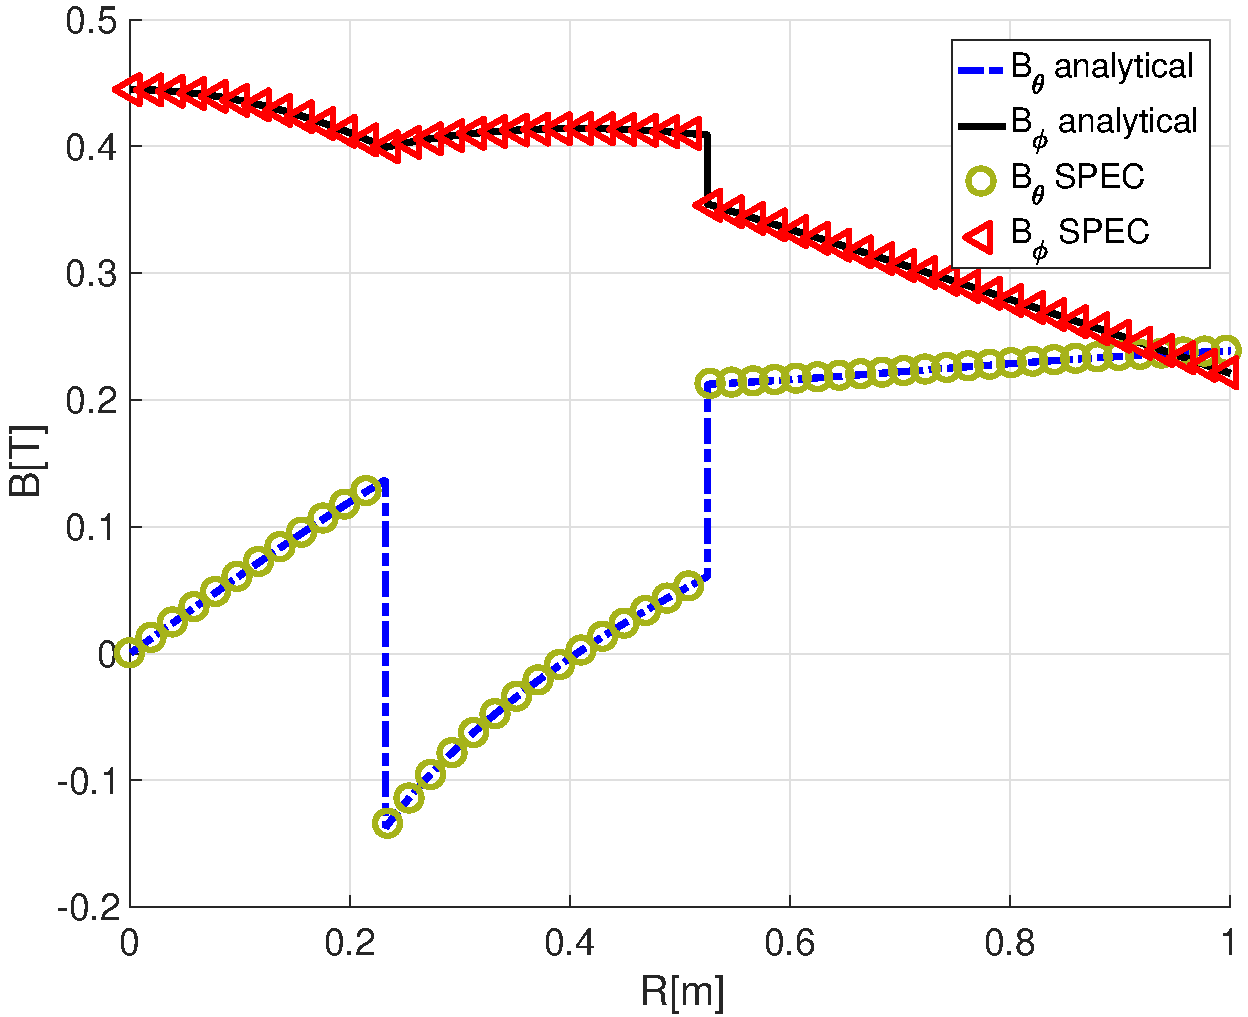
\includegraphics[width=0.5\linewidth]{main/Figures_CurrentConstraint/ABaillod_fig6.pdf}
	\caption{Magnetic field components as a function of the radius in the case of a screw pinch. Solid and dashed lines: analytical solution as given in Appendix \ref{appB}. Circles and triangles: \ac{SPEC} solution using the current constraint.}
	\label{fig:SP_constraint_verification}
\end{figure}
The force gradient can also be expressed in terms of Bessel functions integrals (see Appendix \ref{appB}). Figure \ref{fig:ForceGradient_Convergence_ScrewPinch} shows the normalized maximum absolute error between the force gradient obtained with \ac{SPEC} and that obtained analytically as a function of the radial resolution $L_{rad}$. As $L_{rad}$ is increased, exponential convergence is observed up until $10^{-13}$, where the error in the evaluation of the Bessel integrals starts to dominate. 

\begin{figure}
	\centering
	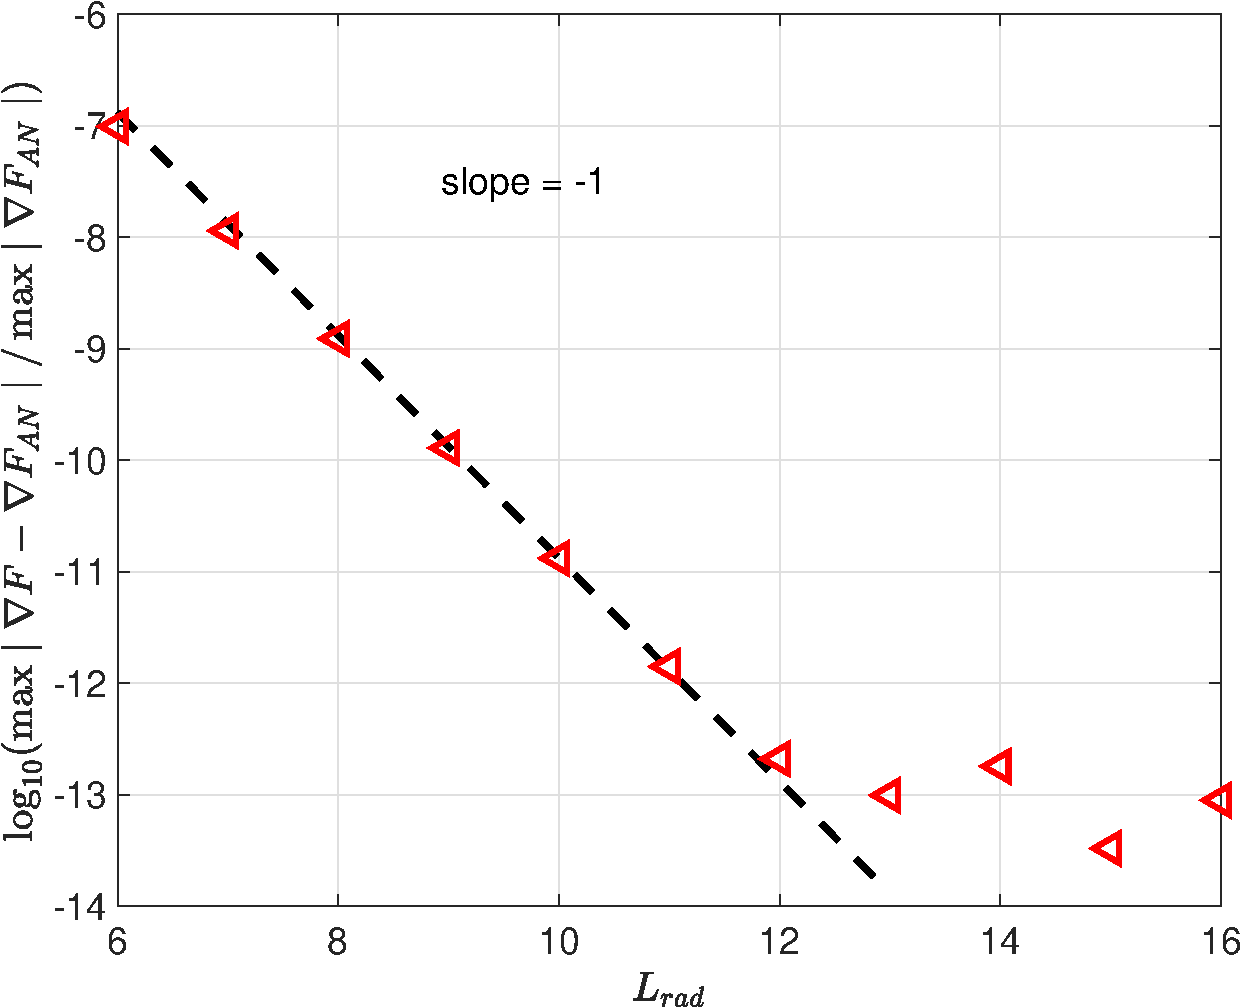
\includegraphics[width=0.5\linewidth]{main/Figures_CurrentConstraint/ABaillod_fig7.pdf}
	\caption{Semi-logarithmic plot of the maximal absolute error between the analytical force gradient, $\nabla F_{AN}$, and the force gradient obtained from \ac{SPEC}, $\nabla F$, as a function of the radial resolution for the screw pinch case.}
	\label{fig:ForceGradient_Convergence_ScrewPinch}
\end{figure}

\subsubsection{Verification in toroidal geometry}

A verification is proposed here in the more complex case of a free-boundary, rotating ellipse (also called classical stellarator) equilibrium with $5$ field periods ($N_p=5$), multiple poloidal and toroidal modes ($M_{pol}=4$ and $N_{tor}=2$) and seven plasma volumes ($N_{vol}=7$). The pressure is set to zero and the computational boundary is defined by

\begin{align}
	R &= R_{00} + R_{10} \cos\theta + R_{11}\cos(\theta - N_p\phi)\label{eq.RotEllipse_R}\\
	Z &= Z_{00} + Z_{10} \sin\theta + Z_{11}\sin(\theta - N_p\phi),\label{eq.RotEllipse_Z}
\end{align}
with $R_{00}=10$m, $Z_{00}=0$m, $R_{10}=-Z_{10}=1$m, $R_{11}=Z_{11}=0.25$m and $N_p = 5$ (see Figure \ref{fig:3Dplot}). We suppose here that some hypothetical coils with a total current of $\mu_0I_{coil}=42.87$Tm are able to generate a vacuum field without normal component to the computational boundary. The total toroidal magnetic flux in the plasma is set to $\psi_a=0.61\text{Tm}^2$ and the toroidal magnetic flux in the vacuum region is set to $\psi_{t,V}=1.39\text{Tm}^2$, adding up to a total toroidal magnetic flux enclosed by the computational boundary of $\psi_{t,V} + \psi_a = 2\text{Tm}^2$.

\begin{figure}
	\centering
	\includegraphics[width=0.5\linewidth]{main/Figures_CurrentConstraint/ABaillod_fig8.pdf}
	\caption{\ac{3D} plot of the classical stellarator boundary as described by Eqs.(\ref{eq.RotEllipse_R})-(\ref{eq.RotEllipse_Z}). Colors indicate the magnetic field strength.}
	\label{fig:3Dplot}
\end{figure}

To the authors knowledge, no analytical solution to Eqs.(\ref{eq.BeltramiEquation}) and (\ref{eq.force_balance}) exists in this geometry. The verification is thus carried out as follows: first, a rotational transform constraint case is run with an input $\iotabar$-profile that is chosen to be $10\%$ larger than the vacuum rotational transform $\iotabar_{vac}$, \textit{i.e.} $\iotabar = 1.10\cdot\iotabar_{vac}$, so that there is a non-zero contribution from the current to the rotational transform. The volume and surface currents are evaluated from the obtained equilibrium and used to run a current constraint calculation to obtain a second equilibrium. The same initial guess for the geometry and the interfaces is used for both calculations. The rotational transform profile $\bar{\iotabar}$ is then extracted from the second equilibrium and compared to the reference $\iotabar$-profile.

The vacuum rotational transform profile, as well as the profiles $\iotabar$ and $\bar{\iotabar}$ are shown in Figure \ref{fig:iota_and_current_profile} (left). The toroidal current enclosed by the plasma is mostly contained in the volumes and adds up to a total of $\sim 2.7$kA, see Figure \ref{fig:iota_and_current_profile} (right). As expected the surfaces currents $I^s_{\phi,l}$ remain small ($<10^{-2}$kA), since there are no pressure gradients to drive them. The constraint on the rotational transform $\iotabar$ is enforced on each side of the volumes' interfaces, indicated by gray dashed lines on Figure \ref{fig:iota_and_current_profile} (left). The value of $\iotabar$ at the computational boundary is not constrained. Agreement between $\iotabar$ and $\bar{\iotabar}$ up to a relative error of $\max(\mid\iotabar-\bar{\iotabar}\mid / \mid\iotabar\mid)\sim 10^{-5}$ is observed, showing that the same equilibrium can be obtained using either constraint. The maximum error between both profiles decreases as the numerical resolution is increased (data not shown).


\begin{figure}
	\centering
	\hfill
	\subfloat[][]{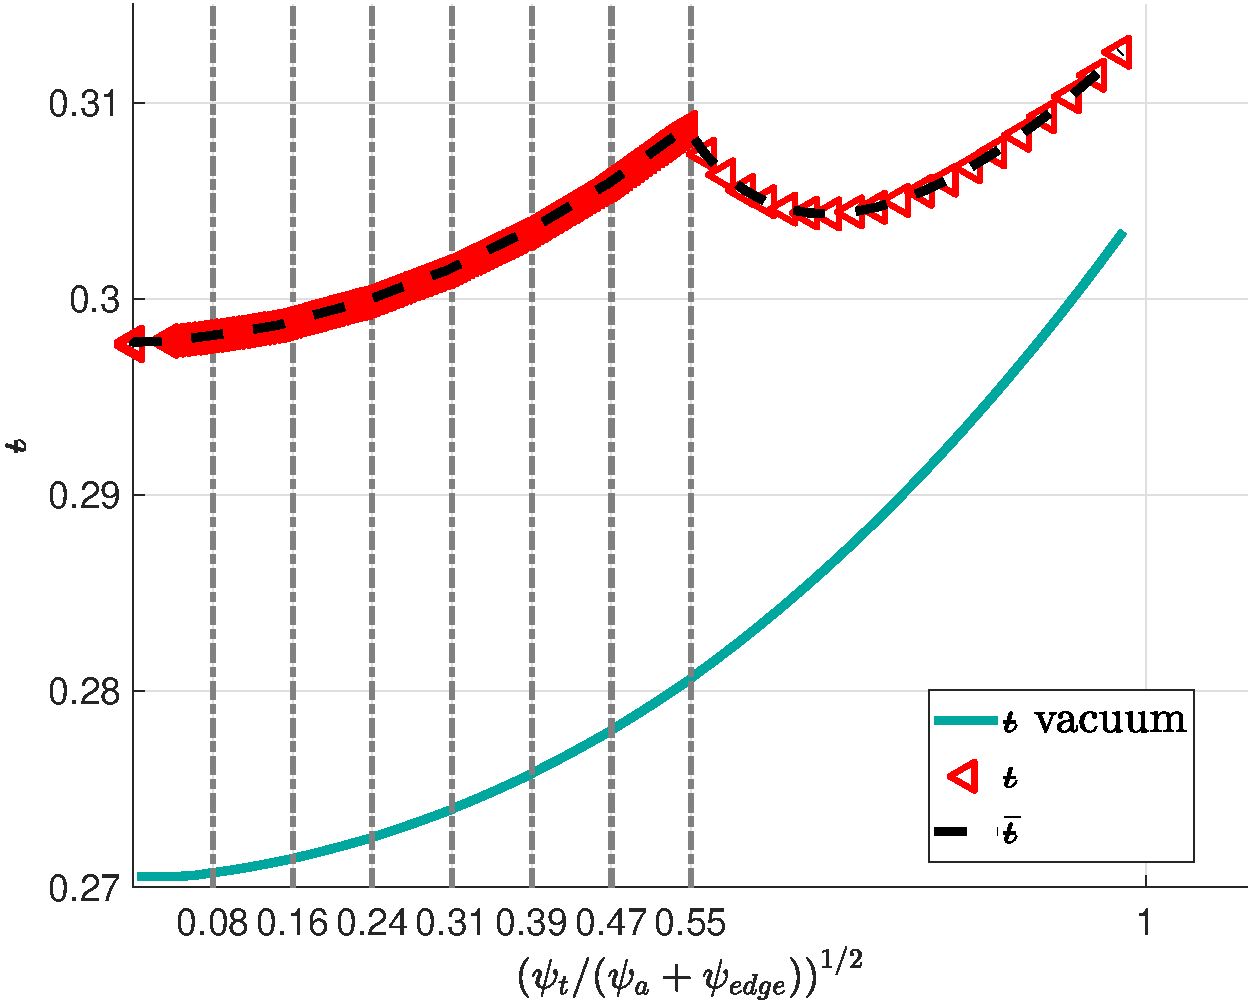
\includegraphics[width=.45\textwidth]{main/Figures_CurrentConstraint/ABaillod_fig9a.pdf}}
	\hfill
	\subfloat[][]{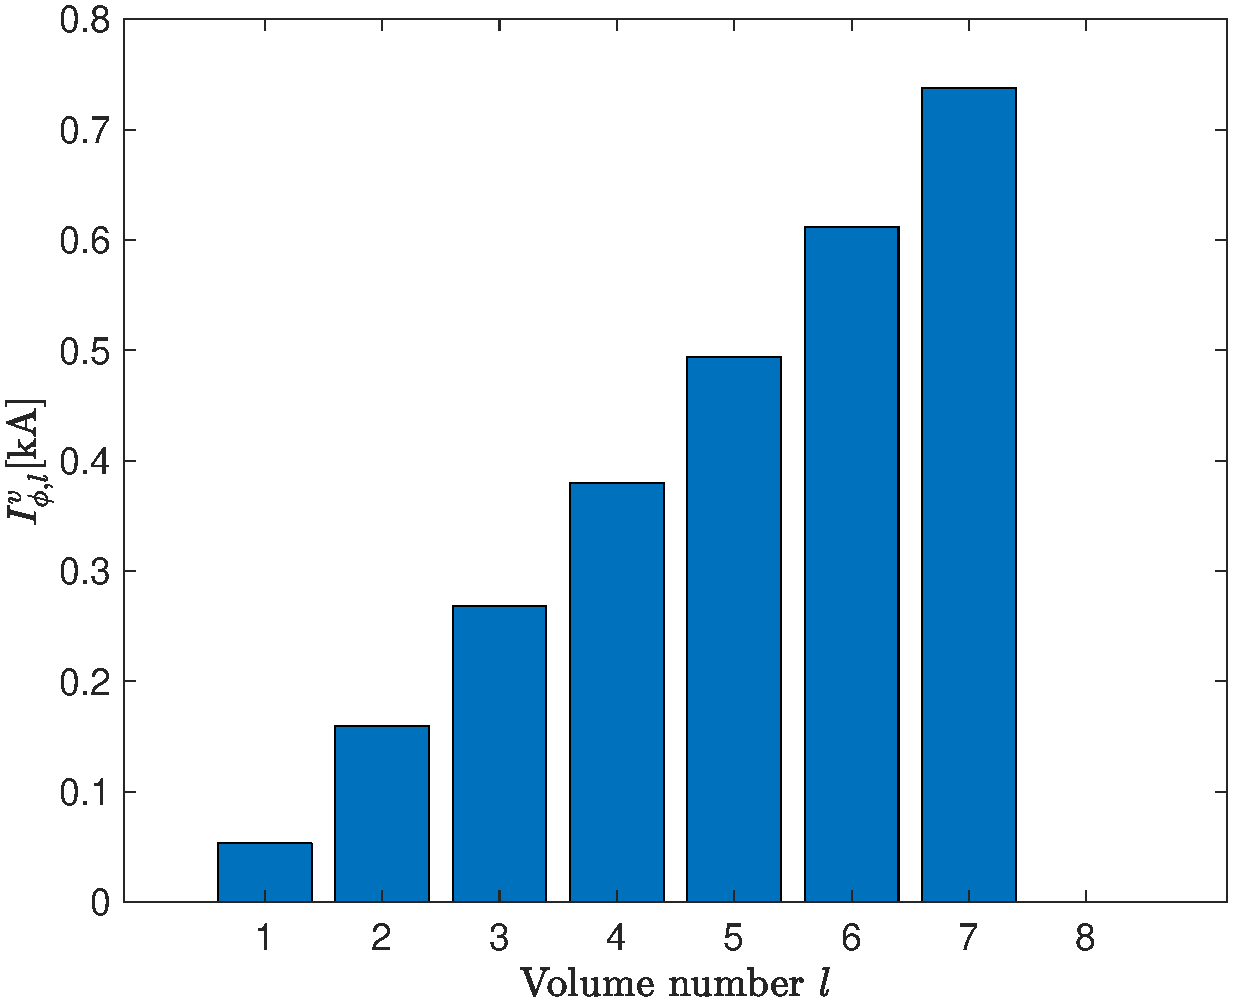
\includegraphics[width=0.45\linewidth]{main/Figures_CurrentConstraint/ABaillod_fig9b.pdf}}
	\hfill
	\caption{Left: rotational transform profile versus effective minor radius. Red triangles: $\iotabar$, input profile used in \ac{SPEC} when run at fixed rotational transform. Black, dashed line: $\bar{\iotabar}$, the output profile obtained from \ac{SPEC} when run at fixed toroidal current profile. Blue line: $\iota$-profile in vacuum. Gray dashed lines: Position of volume interfaces. Right: total toroidal current enclosed by each volume. Surface currents (not plotted), $I^s_{\phi,l}$, are smaller than $10^{-2}$[kA] and are negligible in comparison to the volume current.}
	\label{fig:iota_and_current_profile}
\end{figure}

To verify the force gradient components, we use a fourth-order centered finite difference formula \citep{Fornberg1988},

\begin{equation}
	\frac{d f}{d x} = \frac{f(x-2\Delta x)  - 8f(x-\Delta x) + 8f(x+\Delta x) - f(x+2\Delta x)}{12\Delta x} + \mathcal{O}(\Delta x^4),
\end{equation}
to obtain $\nabla F_{FD}$, \textit{i.e.} a finite-difference estimate of the force gradient, and compare it to $\nabla F$, \textit{i.e.} the force gradient calculated in \ac{SPEC} by using analytical derivatives. The finite difference estimate is evaluated by perturbing each geometrical degree of freedom $\{x_i\}_{l=1,\ldots,N}$ by a constant value $\Delta R$. Convergence as $\Delta R\rightarrow 0$ is shown in Figure \ref{fig:conv_FG_rotell}. A convergence of order $\mathcal{O}(\Delta R^4)$ is observed down to $\sim 10^{-11}$ for $\Delta R\sim 10^{-4}$. For lower values of $\Delta R$, the finite difference approximation error is dominated by round-off error. This shows that the analytical derivatives (the force gradient) is correctly implemented in \ac{SPEC}.

\begin{figure}
	\centering
	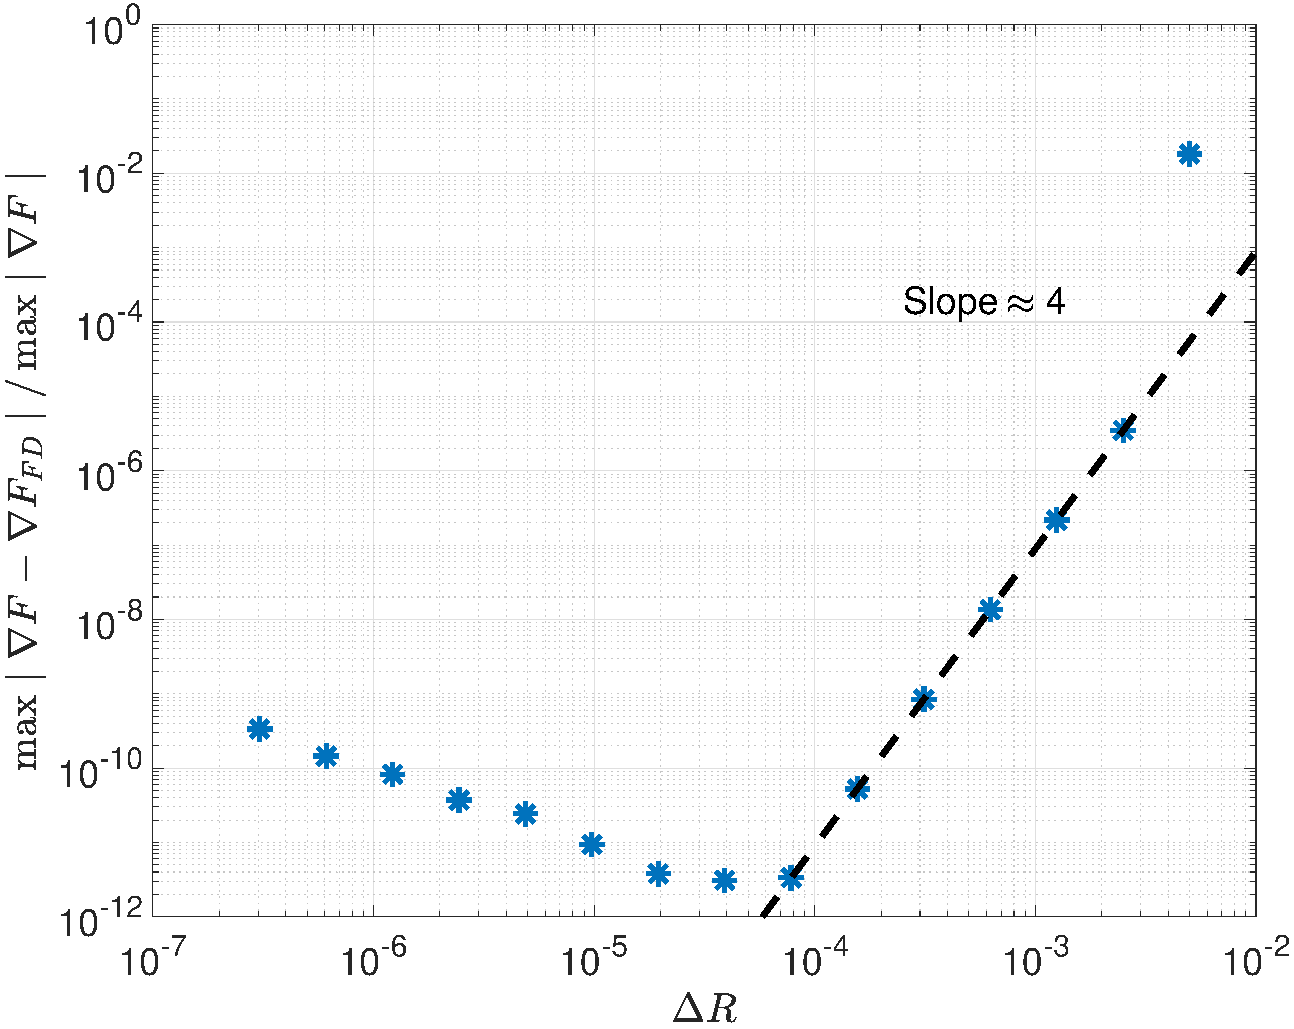
\includegraphics[width=.5\linewidth]{main/Figures_CurrentConstraint/ABaillod_fig10.pdf}
	\caption{Normalized maximum absolute error between \ac{SPEC} force gradient and a finite difference estimate in the case of a rotating ellipse. The dashed line has slope of $4$.} \label{fig:conv_FG_rotell}
\end{figure}




\subsection{Conclusion}

Toroidal currents in \ac{MRxMHD} have been derived and expressed in terms of simple quantities. Two profiles have been identified: the volume current profile, flowing through the volumes, and the surface current profile, flowing at each volume interface. A physical interpretation has been given to each of the currents. Both profiles have been implemented as new constraints in the \ac{SPEC} code, which can now compute \ac{MRxMHD} equilibria for a given toroidal current profile. Analytical derivatives of the force on each volume interface with respect to the interfaces' geometry at fixed toroidal current have been derived and implemented in \ac{SPEC}. These derivatives speed up substantially the Newton iterations on the interface geometries.

Both the new constraint and the force gradient implementation have been verified in slab, cylindrical and toroidal geometries. We presented in this paper only the latter two. In cylindrical geometry, we considered an axisymmetric screw pinch, where the obtained equilibria and force gradient could be compared to analytical solutions. In toroidal geometry, a classical stellarator geometry has been considered. The equilibrium has been verified to match the equilibrium obtained by constraining the rotational transform profile in \ac{SPEC}, and the force gradient has been compared to a finite difference estimate. 


\section{Implementation of a unique angle representation \label{sec. angle representation}}

\subsection{Why a new angle representation is required}
In simple geometries, SPEC provides solutions to the MRxMHD equations in a fast and reliable way. For example, see the studies of \citet{Qu2021,Loizu2020} in slab geometry, or \citet{Kumar2021} in cylindrical geometries or \citet{Kumar2022} in some toroidal geoemtries. However, it is well known by SPEC users that any attempt in strongly shaped geometries will require, at best, a lot of work to help SPEC find a force-balanced equilibrium. In some extreme cases, SPEC does not find an equilibrium, which can either be the case if no solution exist to the equilibrium problem, or if the numerical problem is ill-posed. 


One hypothesis is that the spectral condensation generates many local extrema in the parameter space, which causes the hybrid Powell method used by SPEC not to converge. One solution to this problem would be to choose a suitable poloidal angle $\theta_h$ and thus remove the spectral condensation. In this chapter, we will discuss the implementation of an alternative parametrization for the toroidal surfaces proposed by \citep{Henneberg2021}, which uses such a unique angle. 

\subsection{The Henneberg representation}
One advantageous choice of angle $\theta_h$, called thereafter the \emph{Henneberg angle}, has been proposed by \citet{Henneberg2021}, where they leveraged the fact that magnetic surfaces close to the magnetic axis are ellipses \citep{Helander2014}. The poloidal angle $\theta_h$ is thus chosen to be optimal to represent ellipses. With this angle, a toroidal surface is parametrized by
\begin{eqnarray}
	R(\theta_h,\phi) &= R_0(\phi) + \rho(\theta_h,\phi)\cos(\alpha \phi) - \zeta(\theta_h,\phi)\sin(\alpha \phi), \label{eq.Rfctrhophi}\\
	Z(\theta_h,\phi) &= Z_0(\phi) + \rho(\theta_h,\phi)\sin(\alpha \phi) + \zeta(\theta_h,\phi)\cos(\alpha \phi),\label{eq.Zfctrhophi}
\end{eqnarray}
where $\alpha$ is the number of poloidal rotation of the ellipse per field period --- in general, $\alpha=1/2$. Figure (\ref{sketch Henneberg representation}) shows how the coordinate axis $(\rho,\zeta)$ can be represented. The functions $R_0(\phi)$, $Z_0(\phi)$, $\rho(\theta_h,\phi)$ and $\zeta(\theta_h,\phi)$ are written as

\begin{align}
	\rho(\theta_h,\phi) &= \sum_{m=1}^{M}\sum_{n=-N}^N \rho_{mn}\cos(m\theta_h +n\phi -\alpha \phi),\label{eq.rho_series}\\
	\zeta(\theta_h,\phi) &= b(\phi)\sin(\theta_h-\alpha\phi) =  \sum_{n=0}^N b_n\cos(n\phi)\sin(\theta_h-\alpha \phi), \label{eq.zeta_series}\\
	R_0(\phi) &= \sum_{n=0}^{N} r_n \cos(n \phi)\label{eq.R0_series}\\
	Z_0(\phi) &= \sum_{n=1}^{N} z_n \sin(n \phi)\label{eq.Z0_series}
\end{align}

\begin{figure}
	\centering
	\begin{tikzpicture}
		\node (fig) at (0,0) {
			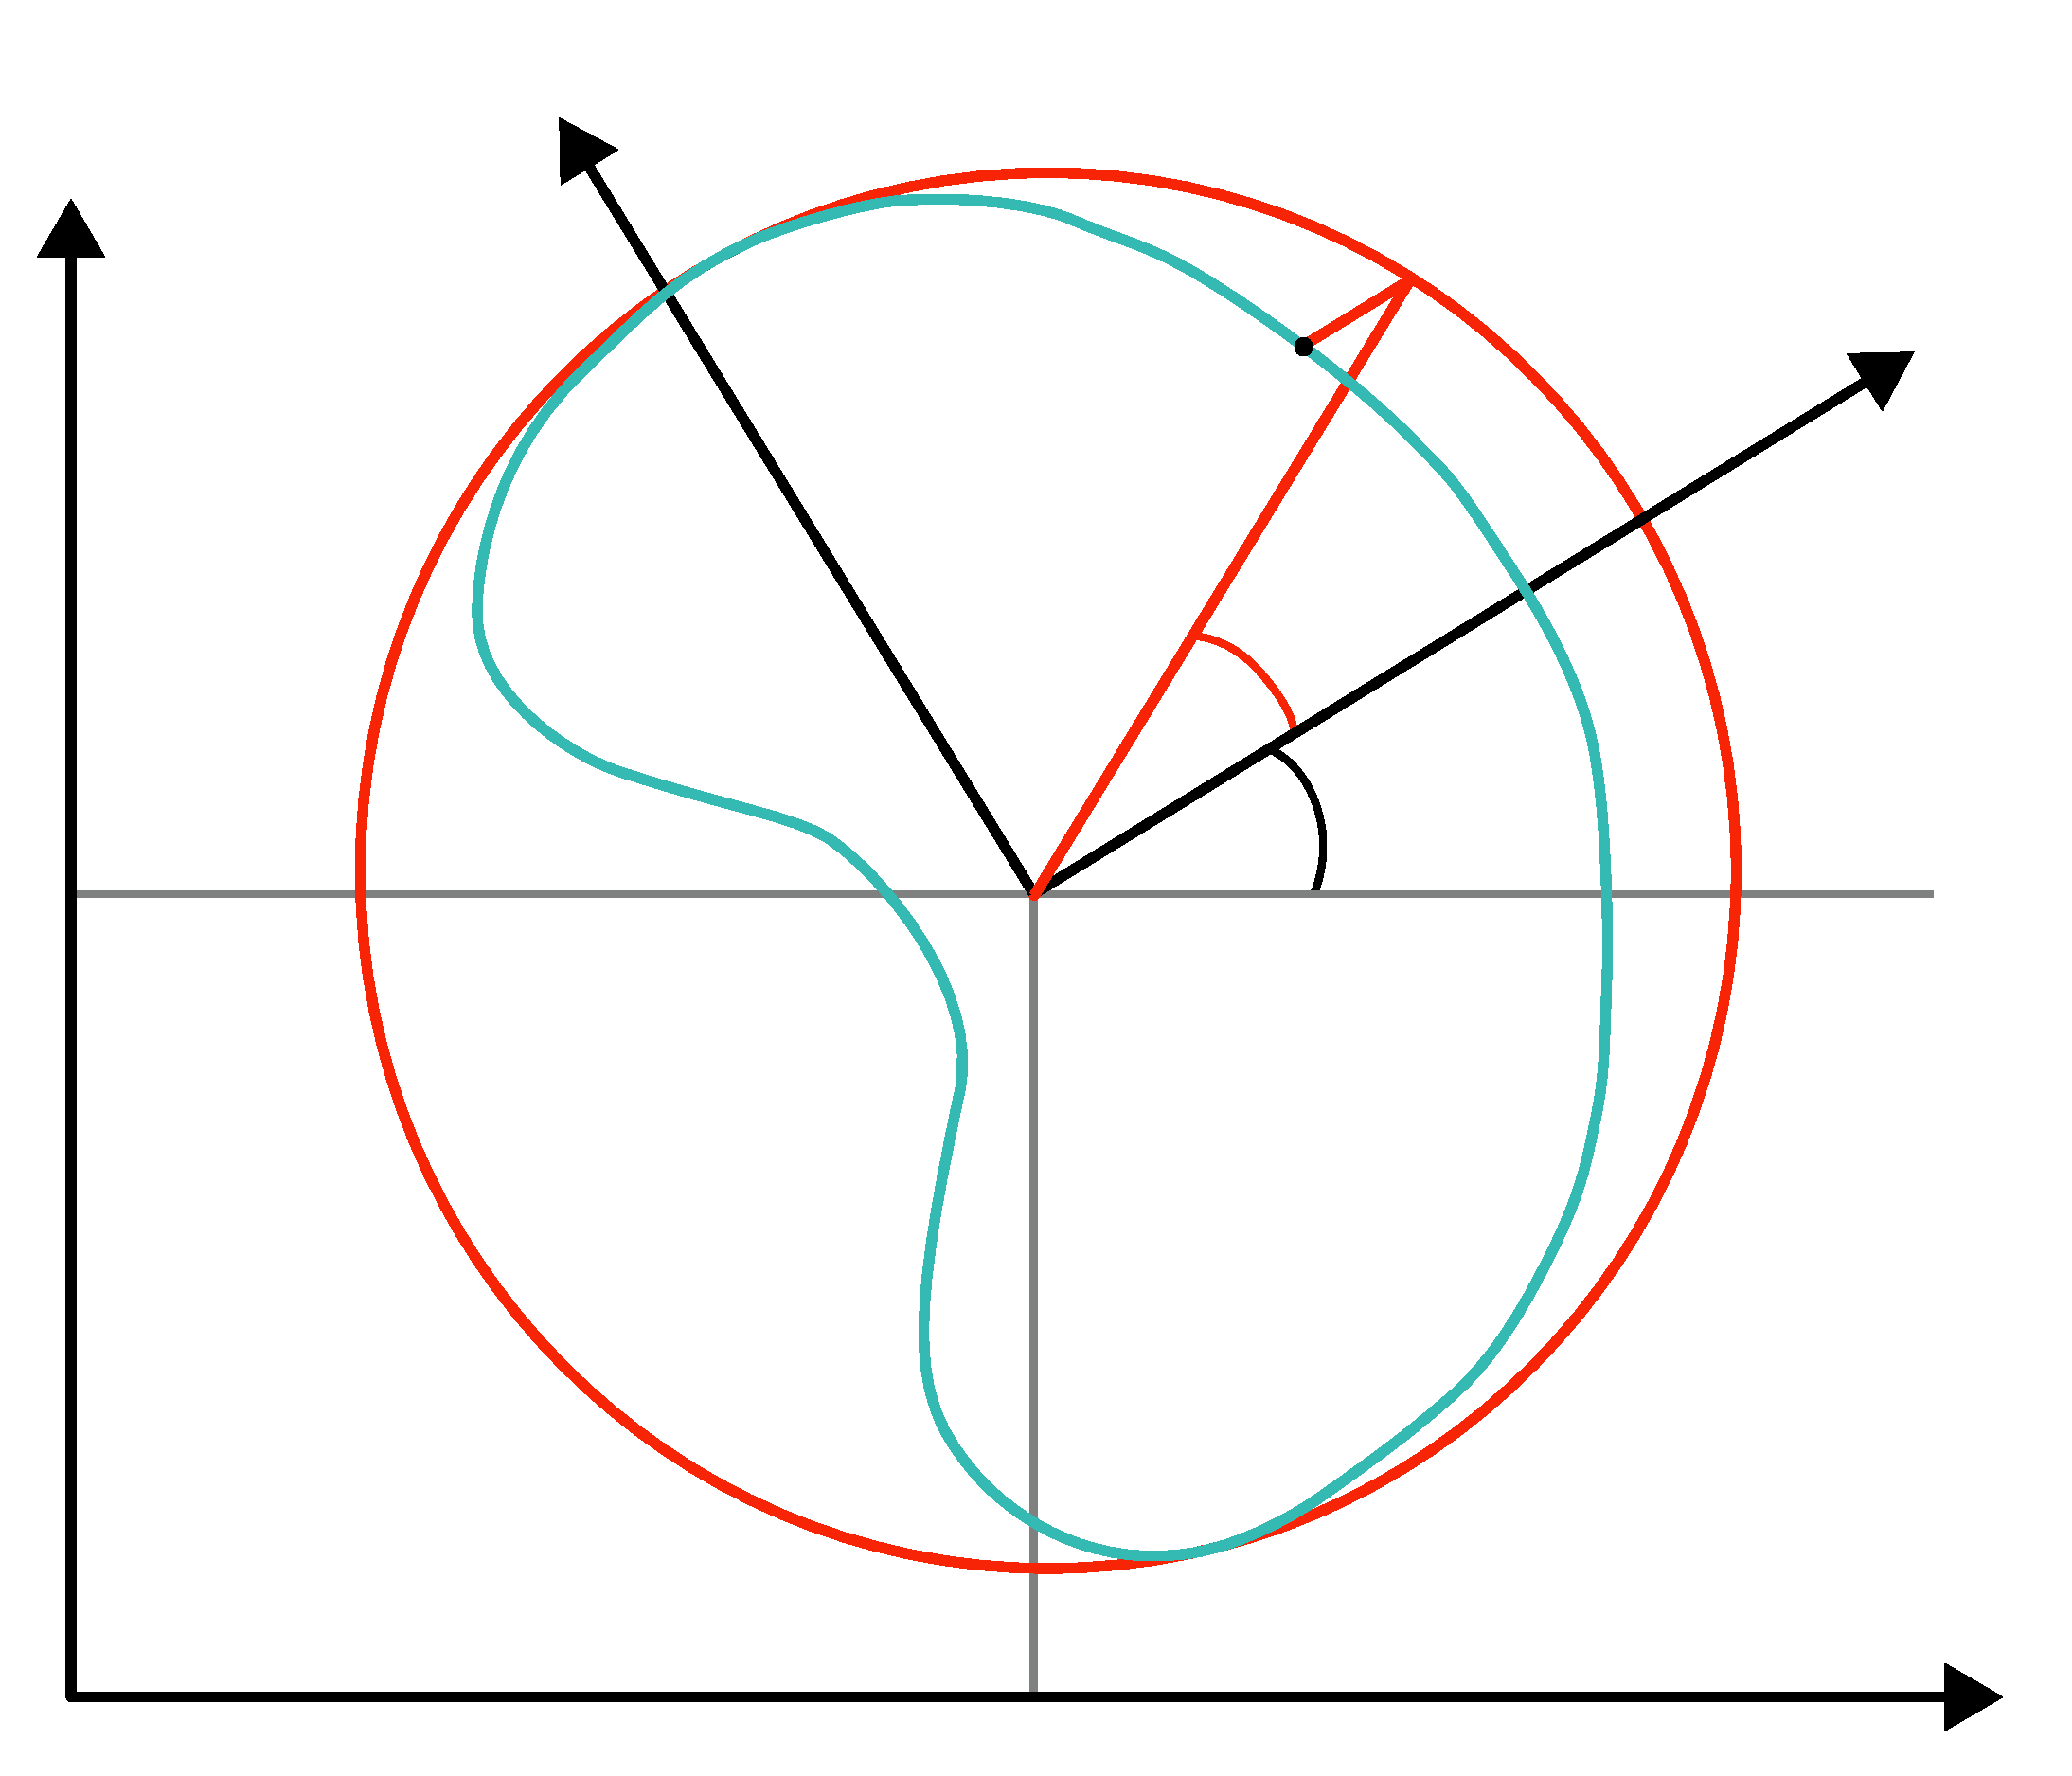
\includegraphics[width=.75\linewidth]{images/HennebergRepresentationSketch}
		};
		\node (Raxis) at (5.1,-3.9) {$\mathbf{e}_R$};
		\node (Zaxis) at (-4.8,3.7) {$\mathbf{e}_Z$};
		\node (Rhoaxis) at (4.6,3.1) {$\mathbf{e}_\rho$};
		\node (Zetaaxis) at (-2.5,4.3) {$\mathbf{e}_\zeta$};
		\node (b) at (.4,1.4) {\color{red}$b(\phi)$};
		\node (theta) at (1.35,1.35) {\color{red}$\theta_h$};
		\node (alphaphi) at (1.9,0.5) {$\alpha\phi$};
		\node (R0) at (-2.1,-0.5) {\color{gray}$R_0(\phi)$};
		\node (Z0) at (.6,-2.1) {\color{gray}$Z_0(\phi)$};
	\end{tikzpicture}
	\caption{Sketch of a toroidal surface (blue) in the $(R,Z)$ plane, and the corresponding coordinates of the Henneberg representation.}
	\label{fig. sketch Henneberg representation}
\end{figure}

The representation given by Eqs.(\ref{eq.Rfctrhophi})-(\ref{eq.Z0_series}) is unique and does not require spectral condensation. Indeed, 
\begin{equation}
	\theta_h = \arcsin\left(\frac{\zeta}{b}\right) + \alpha\phi. \label{eq. henneberg angle}
\end{equation}

One can easily derive a linear relation between the modes $(R_{mn},Z_{mn})$ and the $(r_n,z_n,\rho_{mn},b_n)$. For example, expanding equation (\ref{eq.Rfctrhophi}) with the Fourier series (\ref{eq.rho_series})-(\ref{eq.Z0_series}), we get
\begin{align}
	R(\theta_h,\phi) &= \sum_{n=0}^Nr_n \cos(n \phi) + \sum_{m=1}^{M}\sum_{n=-N}^N \rho_{mn}\cos(m\theta_h +n\phi -\alpha \phi)\cos(\alpha \phi)\\
	&\qquad - \sum_{n=0}^N b_n\cos(n\phi)\sin(\theta_h-\alpha \phi)\sin(\alpha \phi)\\
	&=\sum_{m=1}^{M}\sum_{n=-N}^N \frac{\rho_{mn}}{2}\left[\cos(m\theta_h +n\phi -2\alpha \phi)+\cos(m\theta_h+n\phi)\right]\\
	&\qquad- \sum_{n=0}^N \frac{b_n}{4}\left[\cos(\theta_h-(n+2\alpha)\phi)+\cos(\theta_h-(-n+2\alpha)\phi)\right.\\
	&\qquad\left.-\cos(\theta_h-n\phi)-\cos(\theta_h+n\phi)\right] +  \sum_{n=0}^Nr_n \cos(n \phi),
\end{align}
from which we easily identify
\begin{align}
	R_{0n} &= r_n\\
	R_{mn} &= \frac{1}{2}(\rho_{m,-n+2\alpha}+\rho_{m,-n}) + \frac{\delta_{m1}}{4}\left[b_n+b_-n-b_{n+2\alpha}-b_{n-2\alpha}\right], \qquad \forall m>0. \label{eq, linear relation Rmn}
\end{align}
Similarly, we get
\begin{align}
	Z_{0n} &= z_n\\
	Z_{mn} &= \frac{1}{2}(-\rho_{m,-n+2\alpha}+\rho_{m,-n}) + \frac{\delta_{m1}}{4}\left[b_n+b_-n+b_{n+2\alpha}+b_{n-2\alpha}\right], \qquad \forall m>0.	\label{eq, linear relation Zmn}
\end{align}
Note that to not lose information, the Fourier series of $\rho$ must be truncated at $M=M_{pol}$ and $N=N_{tor}+2\alpha$. Packing the geometrical modes $(R_{mn},Z_{mn})$ in a one dimensional array $\mathbf{x}$ and the modes $(r_n,z_n,\rho_{mn},b_n)$ in another one dimensional array $\mathbf{x}_h$, one can thus write
\begin{equation}
	\mathbf{x}_h = \mathbf{H}\mathbf{x}, \label{eq. henneberg linear system}
\end{equation}
where $\mathbf{H}$ is a matrix of size $(N_h\times N_g)$, with
\begin{align}
	N_h &= 3N + M(2N+1) -1 \\
	&= 3N_{tor} + M_{pol}(2N_{tor}+1) + 4\alpha M_{pol} + 6\alpha N_{tor} -1\\
	N_g & = 2[N_{tor}+M_{pol}(2N_{tor}+1)]+1.
\end{align}
In general, $N_h \neq N_g$, and $\mathbf{H}$ is not a square matrix. In most useful cases ($N$ reasonably large and $\alpha=1/2$), $N_h>N_g$ and the system (\ref{eq. henneberg linear system}) is overdetermined. A solution exist if there is a single maximum and minimum in $\zeta$ for each toroidal plane.

\subsection{Fourier transform}
Note that the relations (\ref{eq, linear relation Rmn}) and (\ref{eq, linear relation Zmn}) assume that the $(R_{mn},Z_{mn})$ are constructed using the same angle $\theta_h$ as the Henneberg representation. The question, then, is the following: given a general surface $(R(\theta,\phi),Z(\theta,\phi))$, how can the Fourier harmonics $(r_n,z_n,\rho_{mn},b_n)$ which describe a surface $(R'(\theta_h,\phi),Z'(\theta_h,\phi))$ and that matches best the input surface be found?

%The starting point is to evaluate the functions $(R(\theta,\phi),Z(\theta,\phi))$ on a sufficient number of grid points $(\theta_i,\phi_j)$, giving $R(\theta_i,\phi_j)\equiv R_{ij}$ and $Z(\theta_i,\phi_j)=Z_{ij}$.
We first construct the function $b(\phi)$. As $b(\phi)$ is independent of $(R_0,Z_0)$, we can set $R_0=Z_0=0$ and identify the poloidal angle $\theta$ that extremizes the $\zeta$ coordinate for each angle $\phi$,
\begin{align}
	\tilde\zeta(\theta_+,\phi) &= \max_{\theta\in[0,2\pi]}\tilde\zeta(\theta,\phi)\\
	\tilde\zeta(\theta_-,\phi) &= \min_{\theta\in[0,2\pi]}\tilde\zeta(\theta,\phi)
\end{align}
with $\tilde\zeta$ the coordinate $\zeta$ if $R_0=Z_0=0$.
\begin{equation}
	\tilde\zeta(\theta,\phi) = \sqrt{R^2+Z^2}\cos\left[\alpha\phi+\arctan\left(\frac{R}{Z}\right)\right].
\end{equation}
Then
\begin{equation}
	b(\phi) = \frac{1}{2}\left[\tilde\zeta(\theta_+,\phi)-\tilde\zeta(\theta_-,\phi)\right],
\end{equation}
As $\max_{\theta\in[0,2\pi]}\zeta(\theta,\phi)=-\max_{\theta\in[0,2\pi]}\zeta(\theta,\phi)=b(\phi)$, the position $(R_0(\phi),Z_0(\phi))$ must be 
\begin{align}
	R_0(\phi) &= \frac{1}{2}\left(R(\theta_+,\phi)+R(\theta_-,\phi)\right)\\
	Z_0(\phi) &= \frac{1}{2}\left(Z(\theta_+,\phi)+Z(\theta_-,\phi)\right).
\end{align}
Finally, the coordinate $\rho(\theta,\zeta)$ can be evaluated by
\begin{equation}
	\rho(\theta,\zeta) = (R-R_0)\cos(\alpha\phi) + (Z-Z_0)\sin(\alpha\phi),
\end{equation}
and the Henneberg angle $\theta_h$ can be evaluated via equation (\ref{eq. henneberg angle}). The Fourier harmonics $(r_n,z_n,b_n,\rho_{mn})$ can then be evaluated by standard Fourier transforms. This method can easily be used to transform inputs that uses the more conventional standard representation to inputs that uses the Henneberg representation. The only free parameter in this transformation is the parameter $\alpha$, that has to be choosen by the user. 

\subsection{Implementation in SPEC}
The Beltrami solver in SPEC (section \ref{spec beltrami solver}) has been implemented using the standard representation. To simplify the required changes, it has been decided to not change the Beltrami solver. Instead, the geometrical degrees of freedom on which SPEC iterates to find force balance are the $\mathbf{x}_h=\{r_n,z_n,b_n,\rho_{mn}\}$ harmonics. Then, before entering the Beltrami solver, the mapping (\ref{eq. henneberg linear system}) is applied to get the corresponding $\mathbf{x}=\{R_{mn},Z_{mn}\}$ harmonics. Once the force has been evaluated, a new iteration on the geometry can be made by changing the $\mathbf{x}_h$ harmonics. No backward map from the standard representation to the Henneberg representation is required.

Note that the matrix $\mathbf{H}$ is independent of the geometry, and can be evaluated once at the beginning of SPEC execution. This is of course very advantageous for keeping SPEC speed.

The force gradient, \textit{i.e.} the derivatives of the force Fourier harmonics $F_j$ with respect to the harmonics $(r_n,z_n,b_n,\rho_{mn})$, can be easily obtained by applying the chain rule,
\begin{equation}
	\frac{dF_j}{dx_{h,i}} = \frac{dF_j}{dx_k}\frac{\partial x_k}{\partial x_{h,i}},
\end{equation}
where the matrices elements $dF_j/dx_k$ are the force gradient computed using the standard representation, described in section \ref{sec. force gradient}, and the matrices element $\partial x_k/\partial x_{h,i}$ are obtained by taking the derivative of equation (\ref{eq. henneberg linear system}).

Finally, one has to be careful about the truncation of the Force in Fourier space. The hybrid Powell method used to iterate on the interfaces geometry requires the same number of degrees of freedom as equations, \textit{i.e.} the force must be truncated such that it has $N_h$ Fourier harmonics. This is possible if $m\leq M^f_{pol}= M_{pol}+1$ and $|n|\leq N^f_{tor}= N_{tor}$. The magnetic field and vector potential are, however, still truncated at the same resolution as the standard representation, $M_{pol}$ and $N_{tor}$.


\subsection{Verification and comparison }


\section{Conclusion \label{sec. chap3 - conclusion}}



\end{document}